Spectroscopy results obtained using the echo-root-Lorentzian pulse, together
with standard square and root-Lorentzian pulses for comparison, are shown in
Fig.~\ref{fig:fig2}.  Independent measurements on qubit \CoherenceQubit{} on
\CoherenceDate{} give
$T_1=\MeasuredTOne~\mu\mathrm{s}$ and a Ramsey time
$T_2^*=\MeasuredTTwoStar~\mu\mathrm{s}$ (Supplemental Table~S1).  No
Hahn-echo decay was acquired for this data set, so the Letter does not assign
the Ramsey result to a measured Hahn-echo $T_2$.  For a conservative
measurement-linked transverse reference, we set
$T_{2,\mathrm{eff}}=T_2^*=\EffectiveTTwo~\mu\mathrm{s}$, corresponding to
$1/(\pi T_{2,\mathrm{eff}})=\EffectiveCoherenceFwhm~\mathrm{kHz}$.  The guide
lines in the cached spectroscopy panels instead reflect the historical
simulation inputs documented in Supplemental Table~S1 and are not independent
Hahn-echo evidence.

Square pulses exhibit pronounced power broadening even at low drive
amplitudes compared to Lorentzian-type pulses, with substantial linewidth
expansion observed over three orders of magnitude in amplitude.  In contrast, the root-Lorentzian pulse displays the characteristic power-narrowing behavior and maintains a narrow linewidth. However, for pulse durations comparable to the qubit lifetime $T_1$, coherent oscillations arise for both square and root-Lorentzian pulses,
resulting in amplitude-dependent linewidth variations that hinder precise
spectral extraction.

Introducing a $\pi$ phase inversion at the peak of the root-Lorentzian envelope partitions the drive into two sequential segments of opposite phase, such that the corresponding forward and backward evolutions cancel exactly at zero detuning. This echo-like structure suppresses resonant Rabi oscillations while preserving the off-resonant spectral response, producing a sharp depletion feature centered at the qubit transition frequency. In the frequency domain (Fig.~\ref{fig:fig1}), this manifests as a splitting of the spectral response accompanied by a null at resonance, rendering the measured linewidth largely insensitive to drive amplitude. This mechanism can be viewed as a Loschmidt-echo-like evolution, in which reversibility is achieved only on resonance, while detuning or decoherence breaks the cancellation and restores excitation~\cite{Gorin_2006,PhysRevA.30.1610}. Combined with the adiabatic following ensured by the Lorentzian envelope, this interference effect suppresses both power broadening and coherent Rabi oscillations, enabling narrow spectroscopy over a broad range of drive strengths and with pulse durations substantially shorter than those required by standard spectroscopy or Ramsey interferometry.

Fig.~\ref{fig:fig3} shows a numerical simulation of the qubit state evolution during the spectroscopy echo-root-Lorentzian sequence. At resonance, where the adiabatic condition breaks down, coherent Rabi oscillations are induced by the drive. However, due to the $\pi$ phase inversion at the pulse maximum, the subsequent segment of the drive reverses the accumulated evolution, resulting in a symmetric cancellation that returns the qubit close to the ground state, limited by relaxation. Measurement-linked calculations use $T_1=\MeasuredTOne~\mu\mathrm{s}$ and $T_{2,\mathrm{eff}}=\EffectiveTTwo~\mu\mathrm{s}$. The archived curve in this figure predates that coherence run and used the historical parameters listed in Supplemental Table~S1; it has not been relabeled as a simulation of the measured qubit.

For detuned drives, the system remains in the adiabatic regime throughout most of the pulse duration and undergoes excitation only in the vicinity of the pulse peak, where the phase inversion occurs. In this case, the evolution does not cancel and results in a net population transfer followed by relaxation. As a consequence, different detunings produce distinguishable final states, forming the basis of the spectroscopic response.

% Introducing a sign inversion in the root-Lorentzian envelope produces
% an effective $\pi$ phase shift in the drive, leading to a splitting of the
% carrier frequency in the spectral domain. The resulting Fourier spectrum is approximately flat in the vicinity of the qubit transition while exhibiting a null at resonance (see Fig.. This spectral structure implies that, when scanning the drive frequency, the measurement effectively probes a depletion response: excitation is suppressed at resonance and enhanced off-resonantly, producing a spectroscopic “shadow” centered at the transition frequency. In this sense, the qubit response is inferred from the absence of excitation rather than its presence.

\begin{figure}
    \centering
    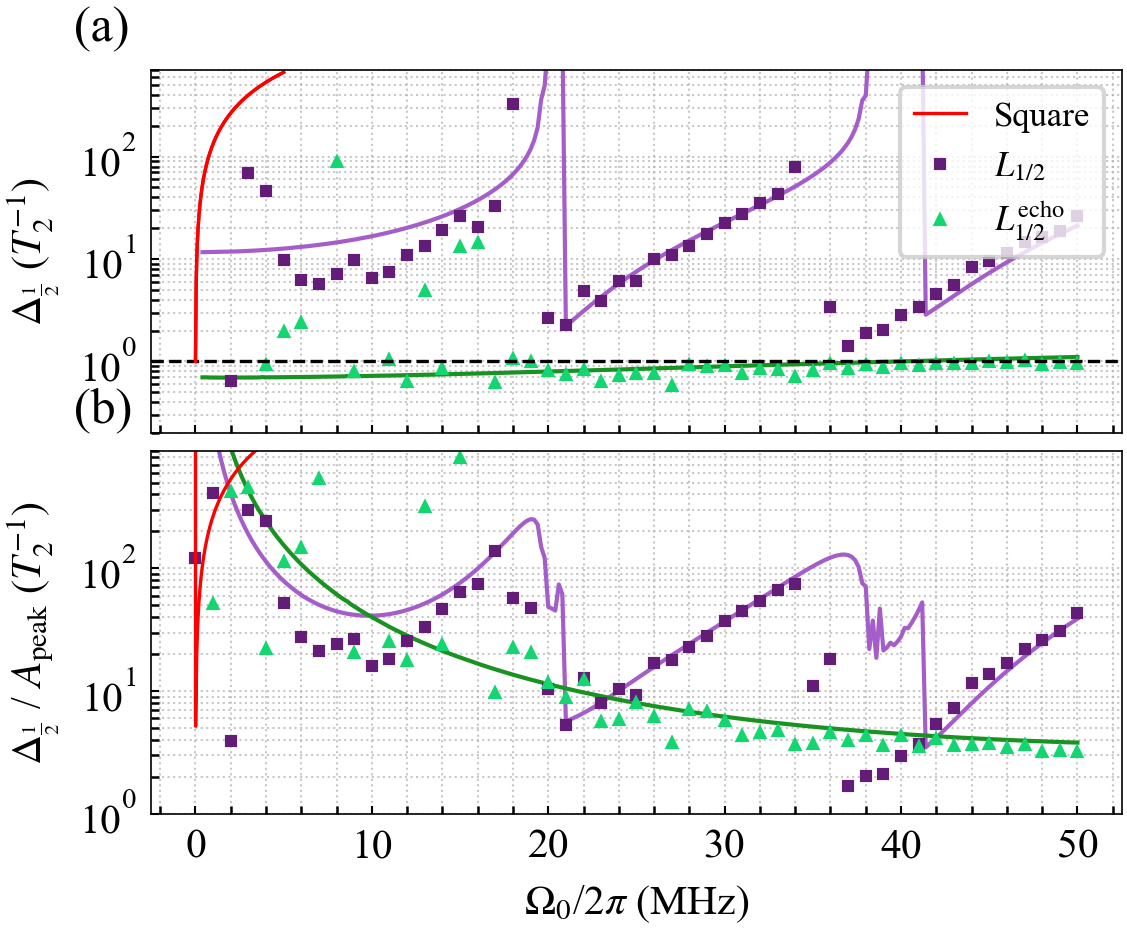
\includegraphics[width=1\linewidth]{figures/fwhm_vs_rabi_prl.png}
    \caption{
    Comparison of spectroscopic linewidth obtained using a constant (square), Lorentzian $L^{(1/2)}$, and echo-Lorentzian $L_{\text{echo}}^{(1/2)} $ drive as a function of peak Rabi frequency $\Omega_0$.
    (a) Measured full width at half maximum (FWHM) $\Delta_{1/2}$ of the qubit spectral response, normalized to the historical model-coherence scale, together with numerical simulations. Solid lines denote simulation results, while markers represent experimental data. The constant drive (red) exhibits conventional power broadening $\Delta_{1/2}\propto\Omega_0$, whereas the Lorentzian (green) and echo-Lorentzian (purple) pulses display power narrowing due to adiabatic following.
    (b) Linewidth-to-signal ratio $\Delta_{1/2}/A_{\text{peak}}$, highlighting the improved resolution--signal trade-off enabled by the echo-Lorentzian protocol at increasing drive amplitude.
    }

    \label{fig:fig4}
\end{figure}

% This mechanism is conceptually analogous to the principle underlying STED microscopy, in which a doughnut-shaped depletion beam suppresses fluorescence everywhere except at a nanoscale central node where the intensity vanishes. By scanning this engineered intensity null across the sample, fluorescence is confined to a sub-diffraction region, enabling spatial resolution beyond the diffraction limit.

% Moreover, this phase-inverted variant structure closely resembles a Loschmidt-echo–type protocol, which quantifies the reversibility of quantum dynamics under perturbations \cite{Gorin_2006,PhysRevA.30.1610}. The echo signal is defined as
% \begin{equation}
% M(t) = \left| \langle \psi_0 | e^{-i H_2 t} e^{-i H_1 t} | \psi_0 \rangle \right|^2,
% \end{equation}

% where  $H_1$  and $H_2$ denote the forward and backward Hamiltonians, respectively. Perfect time reversal ($H_2 = H_1$) yields $M(t) = 1$, while deviations—arising from detuning or noise—lead to a decay governed by decoherence processes. In our implementation, $H_1$ and $H_2$ correspond to two sequential drive segments of opposite phase, such that full reversibility is achieved only at zero detuning.
  


% Second, the echo property, implemented via a $\pi$ phase inversion at the peak of the pulse, acts as a coherent refocusing mechanism. Whereas a standard Lorentzian pulse ultimately suffers from power broadening with increasing drive strength, the phase jump reverses the accumulated phase at resonance and splits the spectral response. As a result, a destructive interference condition emerges at the carrier frequency: only at zero detuning does the forward and backward evolution cancel exactly, giving rise to a sharp and amplitude-robust null—a spectroscopic dark state. 

% The effectiveness of the echo-type Lorentzian pulse arises from two complementary mechanisms. First, the adiabatic nature of the Lorentzian envelope ensures that over a broad range of drive amplitudes the qubit state follows the instantaneous dressed eigenstate of the driven Hamiltonian. In contrast to square pulses—which introduce abrupt non-adiabatic transitions and induce oscillatory Rabi dynamics—the smooth Lorentzian profile suppresses spectral leakage and mitigates the sidebands typically associated with high-power drives.

In Fig.~\ref{fig:fig4}, we plot the extracted spectroscopic linewidth obtained from Gaussian fits to the measured response. Although the spectral lineshape of a driven two-level system is often expected to follow a Lorentzian profile, the interference-based structure of the present protocol results in a more complex response. In this regime, Gaussian fitting provides a robust and consistent estimate of the linewidth while yielding values comparable to those obtained from Lorentzian fits within our resolution requirements.

We compare the experimentally acquired linewidth extracted from two-dimensional frequency–amplitude sweeps with archived numerical simulations of an effective two-level system. The square (red), Lorentzian (green), and echo-Lorentzian (purple) drives are shown, where solid lines denote simulation results and markers represent experimental data. Because the archived curves use the historical coherence inputs in Supplemental Table~S1 rather than the later measured values, the overlay is interpreted qualitatively. For the square pulse, only simulated results are displayed. We plot both the linewidth $\Delta_{1/2}$ and the linewidth-to-signal ratio $\Delta_{1/2}/A_{\mathrm{peak}}$ to quantify the resolution–signal trade-off.

To suppress residual power broadening at large drive amplitudes, the pulse envelope must satisfy requirements on its cutoff behavior. Truncation introduces nonanalytic boundary behavior and a residual cutoff-broadening contribution that scales with the instantaneous amplitude at the cutoff point, denoted $\Omega_c$~\cite{boradjiev_qubit_2013,mihov_defying_2024,mihov_qubit_2024}. In the model, the condition $T_2^{-1}\leq\Delta_{\frac{1}{2}}$ constrains the maximum allowable cutoff amplitude to $\Omega_c<T_2^{-1}$. Empirically, we find that a relative cutoff below $10^{-3}$ suppresses excess cutoff broadening even under strong driving conditions; see the Supplemental Material for the cutoff analysis and high-amplitude measurements~\cite{SupplementalMaterial}.
